\chapter{Oracle Aplication Express}

\section{Tahapan Membuat Aplikasi Akademik Sederhana Oracle Apex}
Pertama kita menormalisasi tabel-tabel yang sudah ada pada bab 3 basisdata semester 1,yakni TAbel MAhasiswa,Dosen,kuliah,Nilai,Jadwal. kita akan langsung mempraktekan bagaimana tahapan pembuatan Aplikasi pada Oracle APEX :

\begin{enumerate}
\item[1]Menormalisasi dan Membuat Tabel Mahasiswa di EXEL. Dengan field NIM,Nama MAhasiswa,Alamat Mahasiswa,Tgl lahir

\begin{figure}[!htbp]
    \begin{center}
    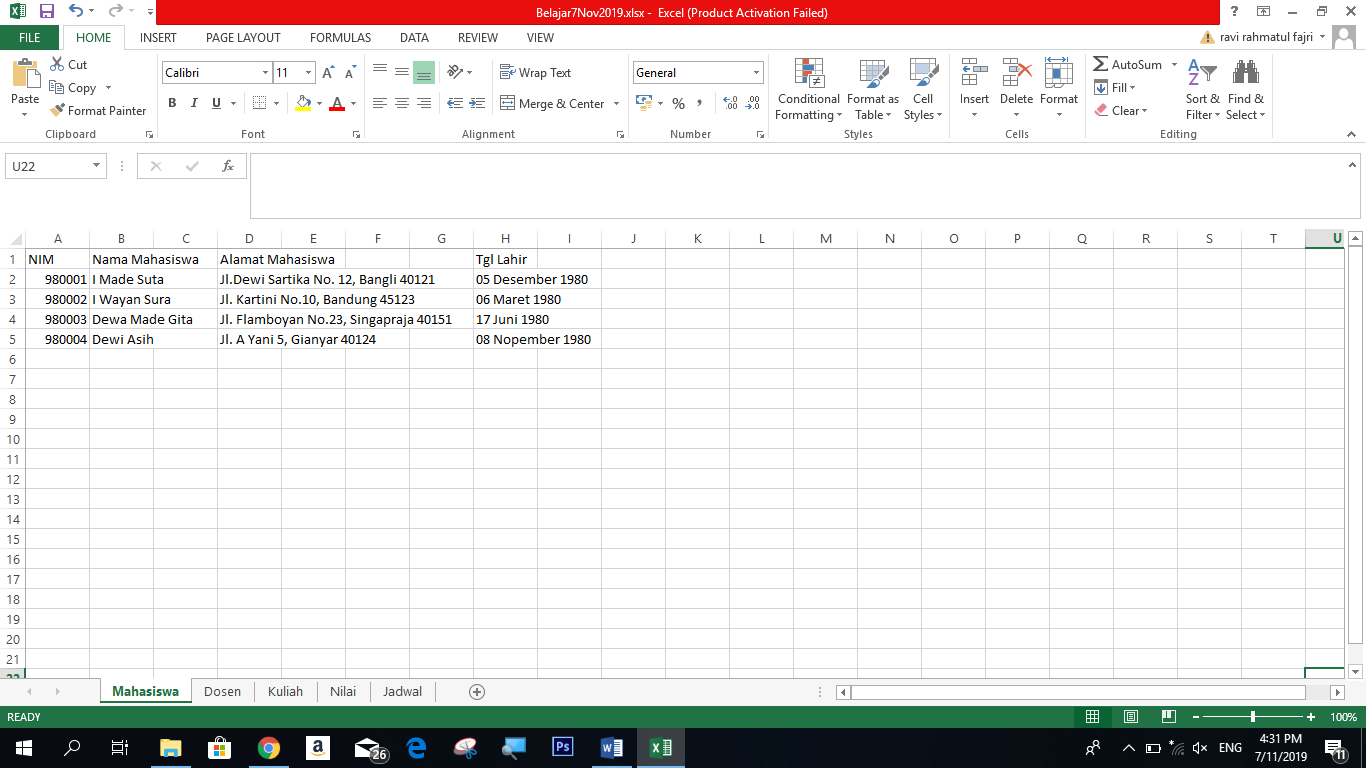
\includegraphics[scale=0.4]{figures/1.png}
    \caption{\textit{Tabel Mahasiswa.}}
    \end{center}   
    \end{figure}

\begin{figure}
\item[2]Menormalisasi dan Membuat Tabel Dosen di EXEL. Dengan Field NIK,Nama Dosen,Akamat Dosen.

    \begin{center}
    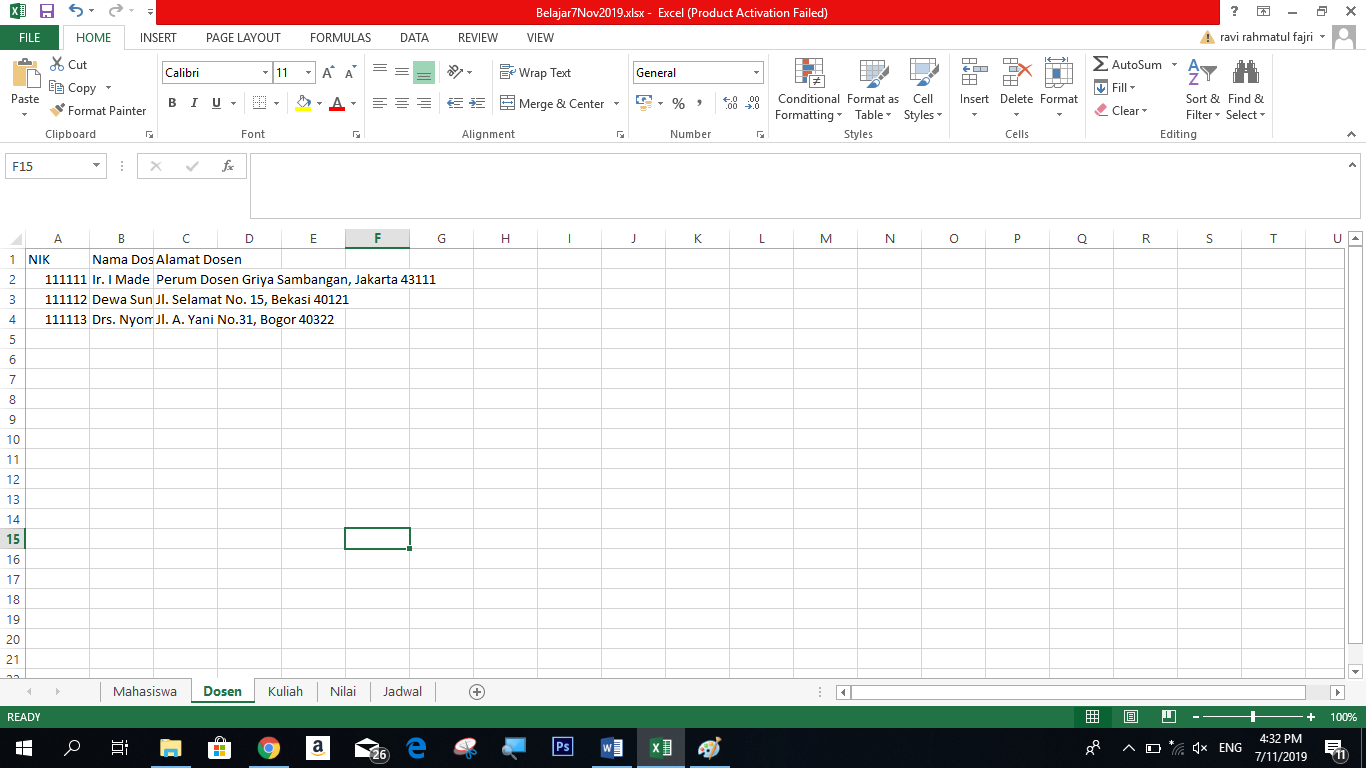
\includegraphics[scale=0.4]{figures/2.png}
    \caption{\textit{Tabel Dosen.}}
    \end{center}
    \label{gambar}
    \end{figure}

\begin{figure}
\item[3]Menormalisasi dan Membuat Tabel Kuliah di EXEL. Dengan Field Kode,SKS,Semester.

    \begin{center}
    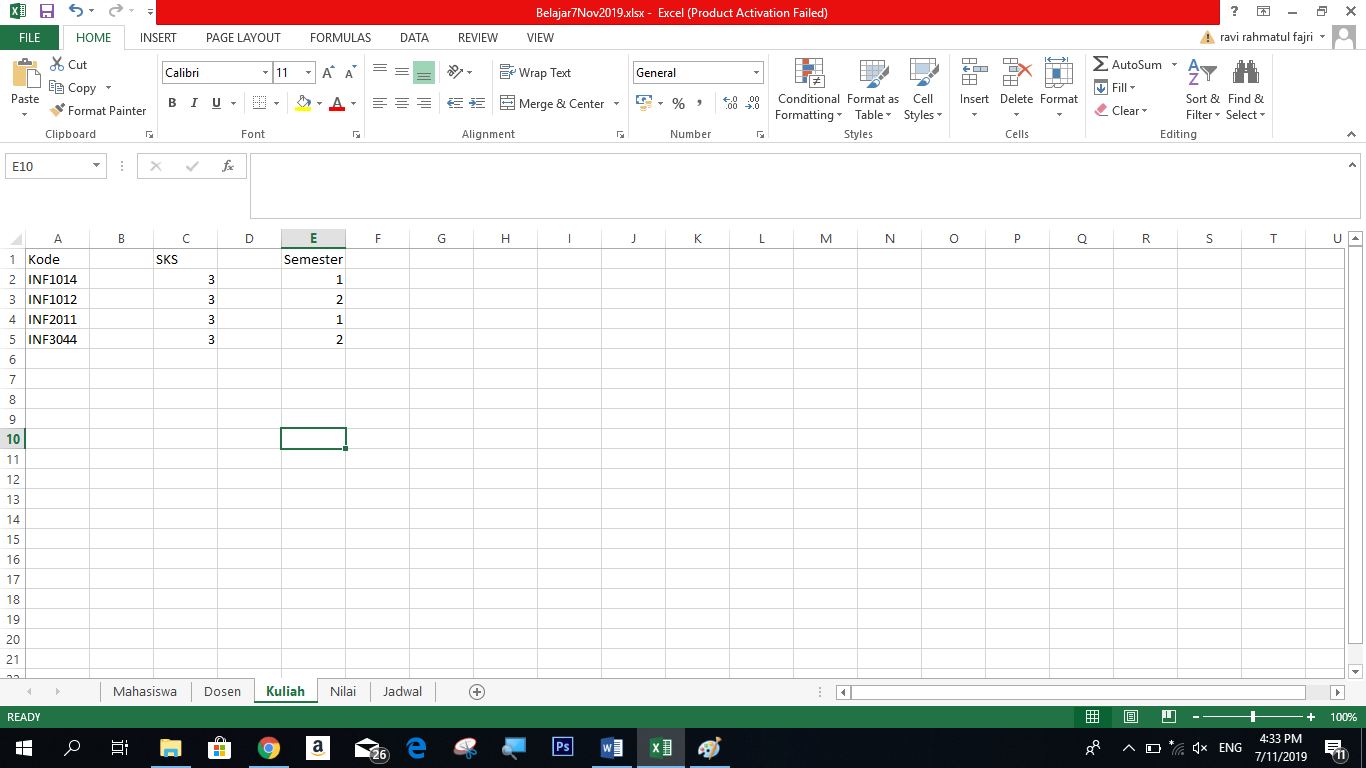
\includegraphics[scale=0.4]{figures/3.png}
    \caption{\textit{Tabel Kuliah.}}
    \end{center}
    \label{gambar}
    \end{figure}

\begin{figure}
\item[4]Menormalisasi dan Membuat Tabel Nilai di EXEL. Dengan Field Kode,NIM,Indeks Nilai. Disini saya salah dalam penulisannya saya menulis Mata Kuliah, akan tetapi sudah saya edit di databasesnya. 

    \begin{center}
    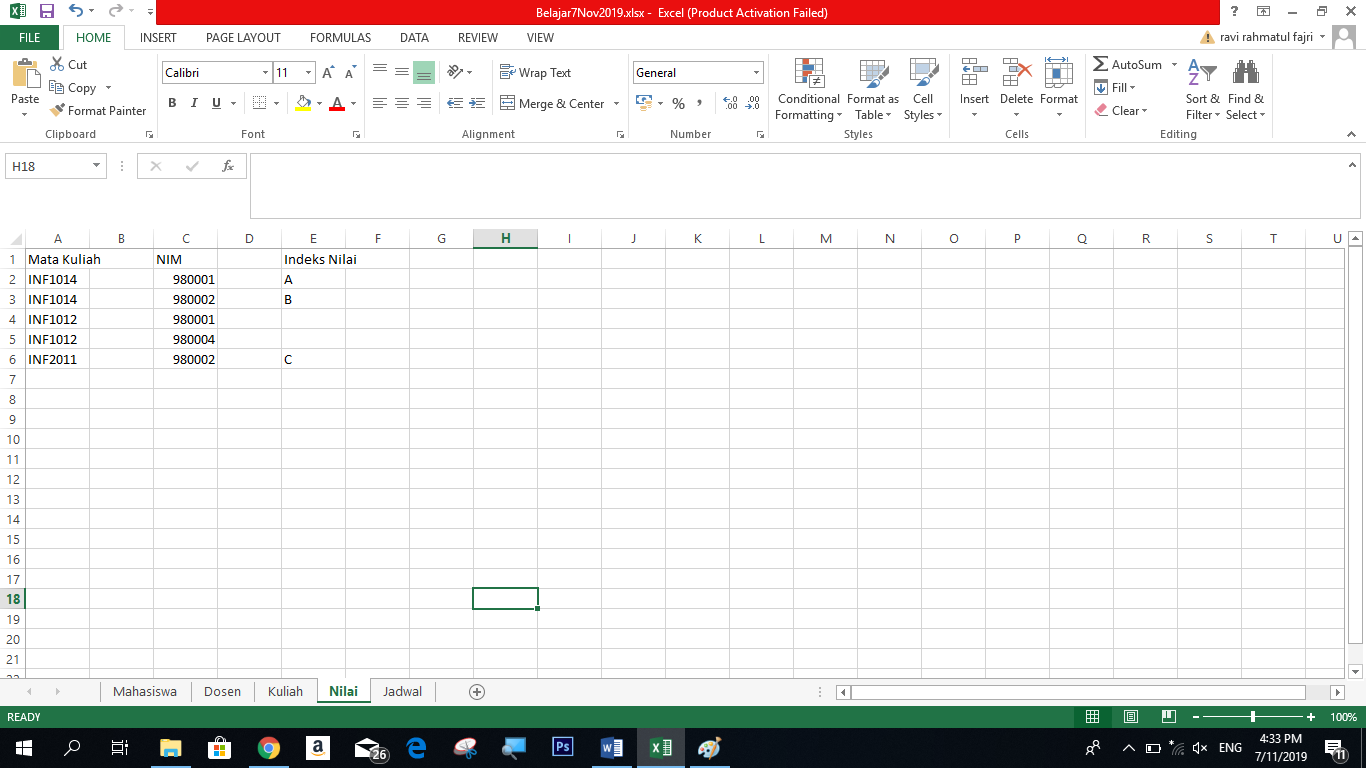
\includegraphics[scale=0.4]{figures/4.png}
    \caption{\textit{Tabel NIlai.}}
    \end{center}
    \label{gambar}
    \end{figure}

\begin{figure}
\item[5]Menormalisasi dan Membuat Tabel Jadwal di EXEL. Dengan Field Kode,Waktu,Tempat,NIK.

    \begin{center}
    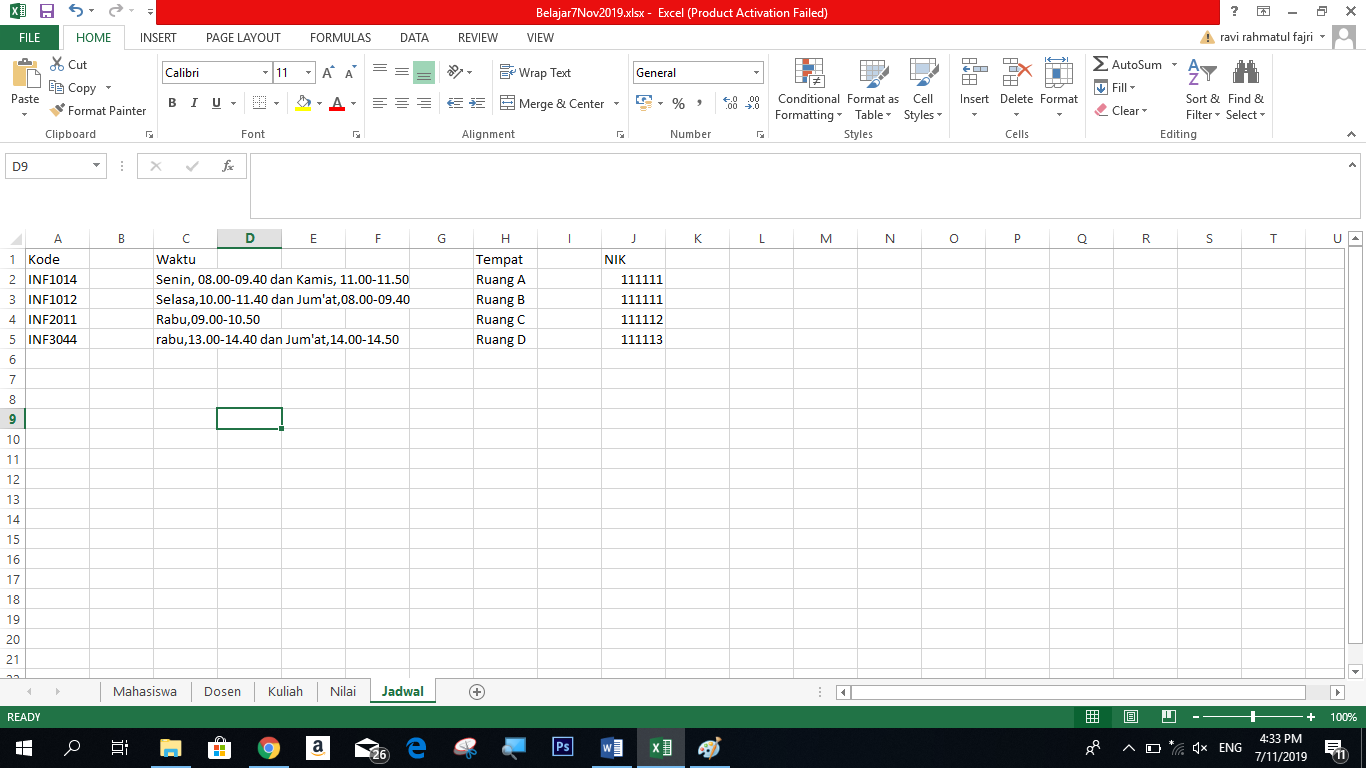
\includegraphics[scale=0.4]{figures/5.png}
    \caption{\textit{Tabel Jadwal.}}
    \end{center}
    \label{gambar}
    \end{figure}

\begin{figure}
\item[6] Setelah Tabel Selesai dibuat, Selanjutnya kita Login

    \begin{center}
    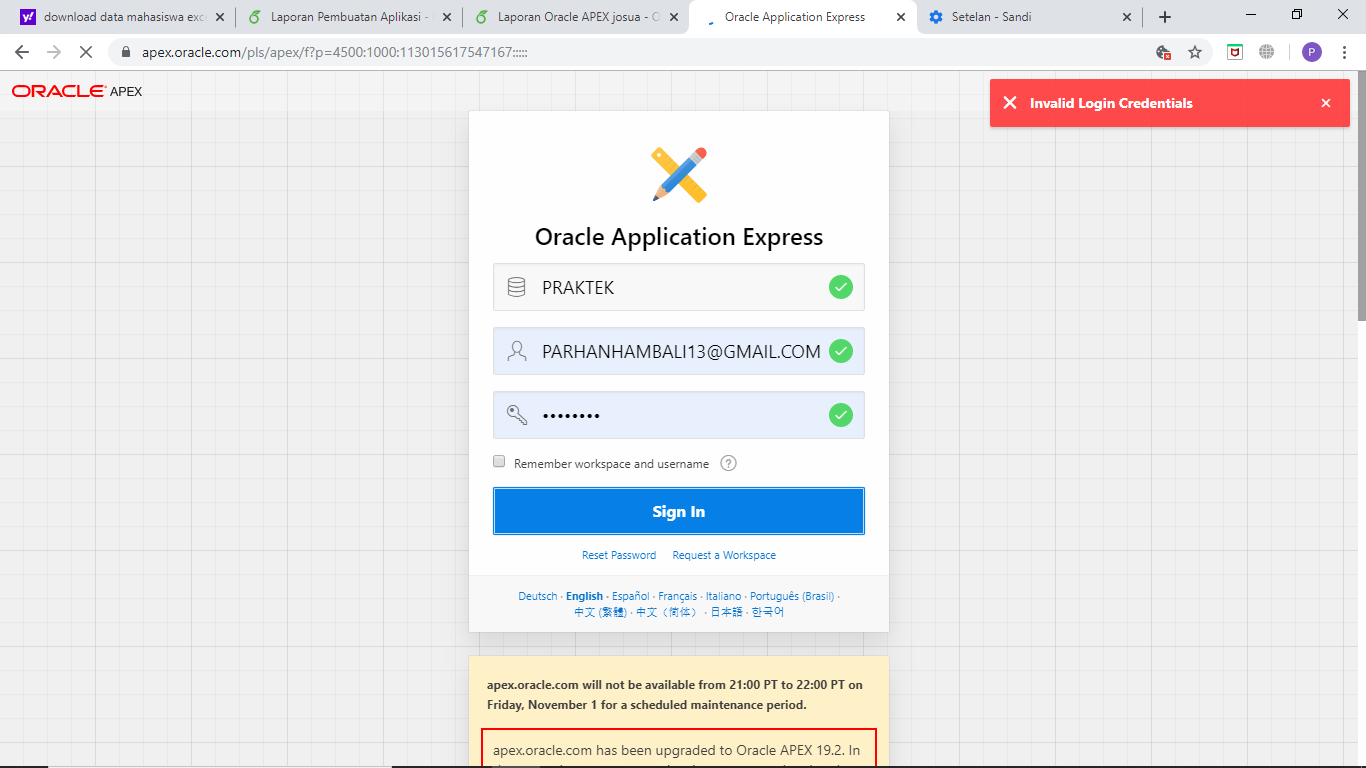
\includegraphics[scale=0.3]{figures/6.png}
    \caption{\textit{Login Apex Online.}}
     \end{center}
    \label{gambar}
    \end{figure}

\begin{figure}
\item[7]Pilih Creat Applikasi

    \begin{center}
    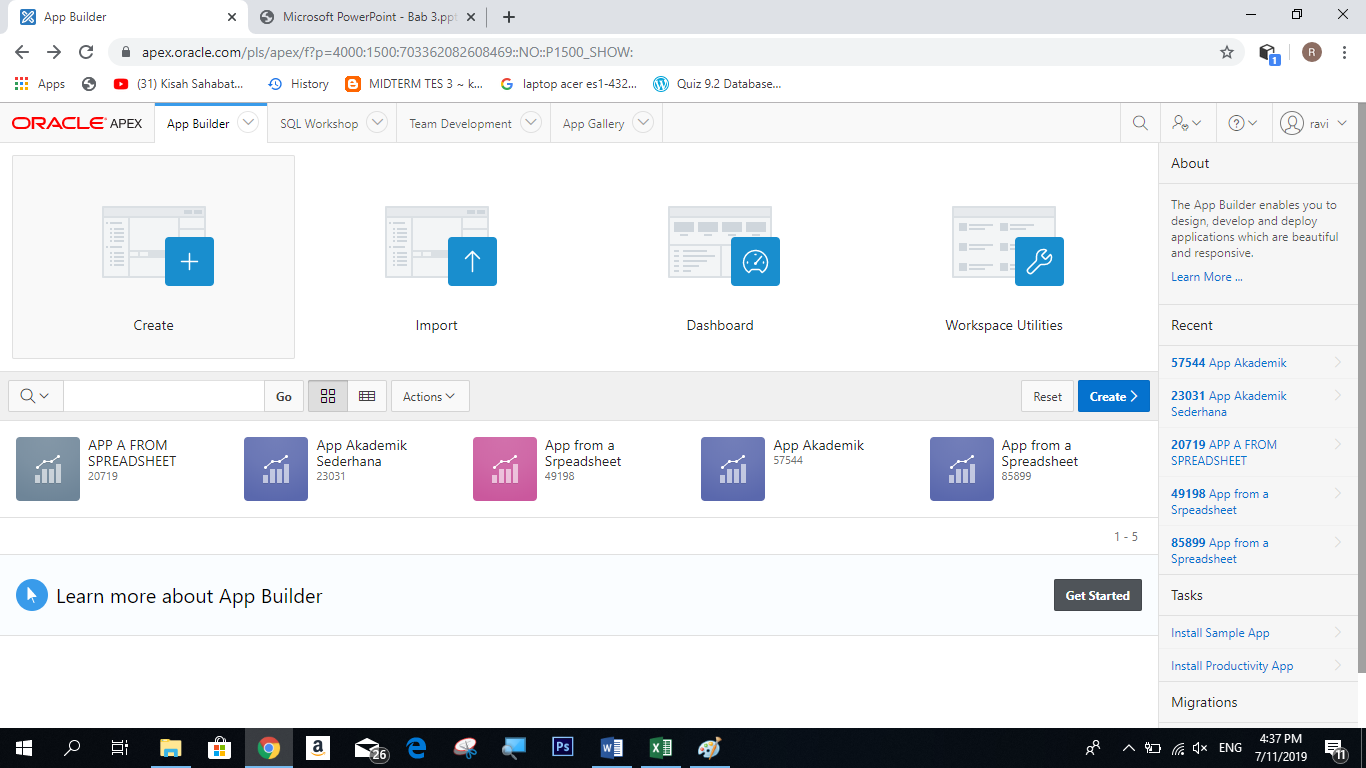
\includegraphics[scale=0.4]{figures/7.png}
    \caption{\textit{Creat Aplikasi.}}
    \end{center}
    \label{gambar}
    \end{figure}

\begin{figure}
\item[8]Pilih From a File, Untuk memasukkan file atau tabel yang telah kita buat tadi yakni dalam bentuk exel.

    \begin{center}
    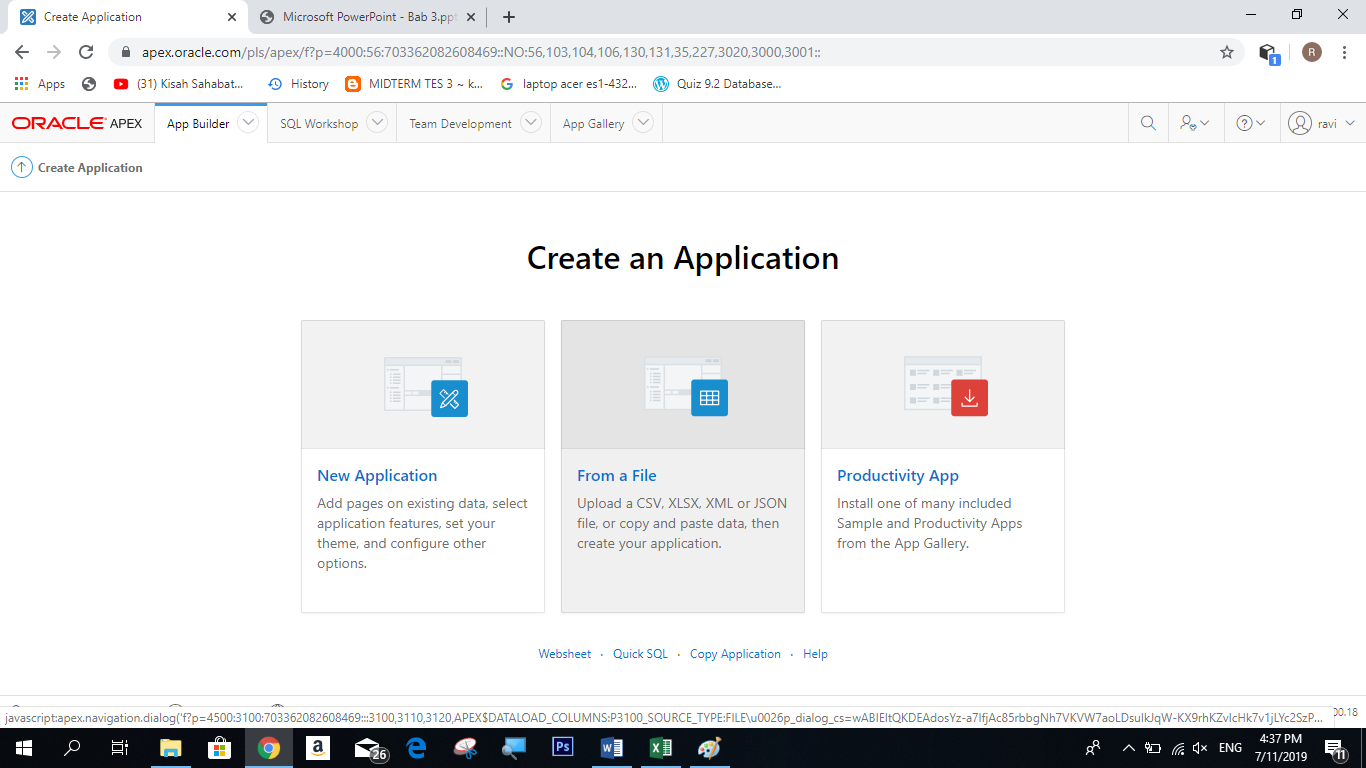
\includegraphics[scale=0.4]{figures/8.png}
    \caption{\textit{From a File.}}
    \end{center}
    \label{gambar}
    \end{figure}

\begin{figure}
\item[9]Choose File atau Pilih file yang telah kita buat tadi

    \begin{center}
    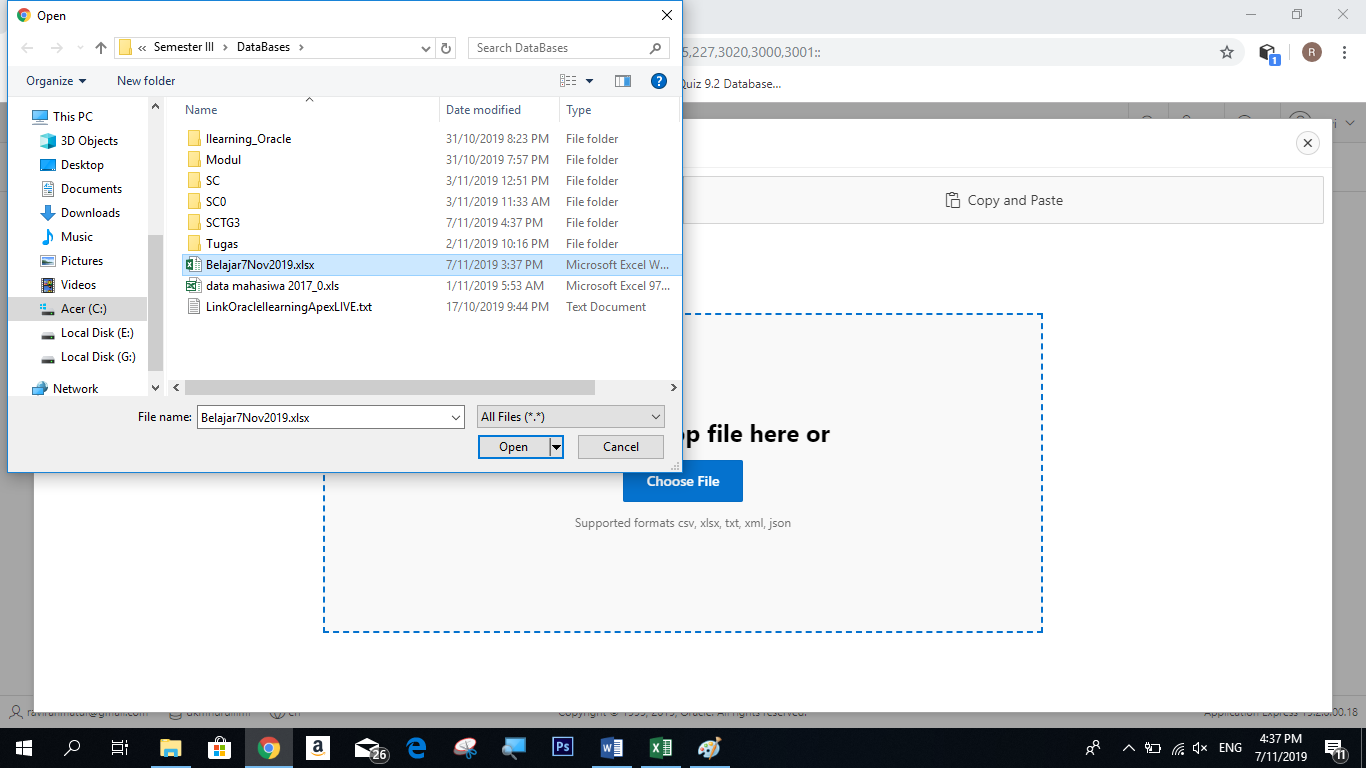
\includegraphics[scale=0.4]{figures/9.png}
    \caption{\textit{Choose File.}}
     \end{center}
    \label{gambar}
    \end{figure}

\begin{figure}
\item[10]Beri nama sesuai urutan tabel tadi, dari yang pertama beri nama tabel Mahasiswa,pastikan select sheet nya sesuai dengan penamaan tabelnya. Selanjutnya Load data

    \begin{center}
    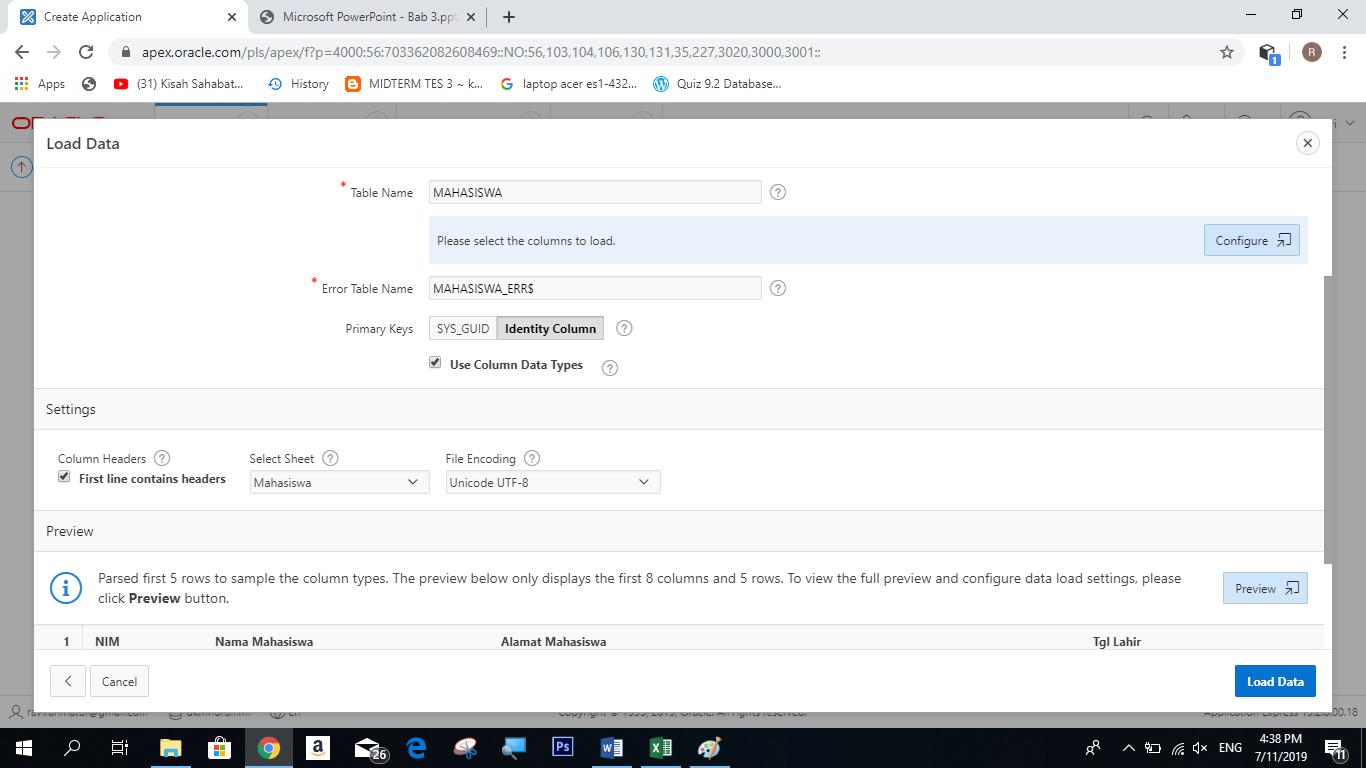
\includegraphics[scale=0.4]{figures/10.png}
    \caption{\textit{Berinama Tabel Mahasiswa.}}
    \end{center}
    \label{gambar}
    \end{figure}

\begin{figure}
\item[11]Beri nama sesuai urutan tabel tadi,Selanjutnya beri nama tabel Dosen,pastikan select sheet nya sesuai dengan penamaan tabelnya. Selanjutnya Load data

    \begin{center}
    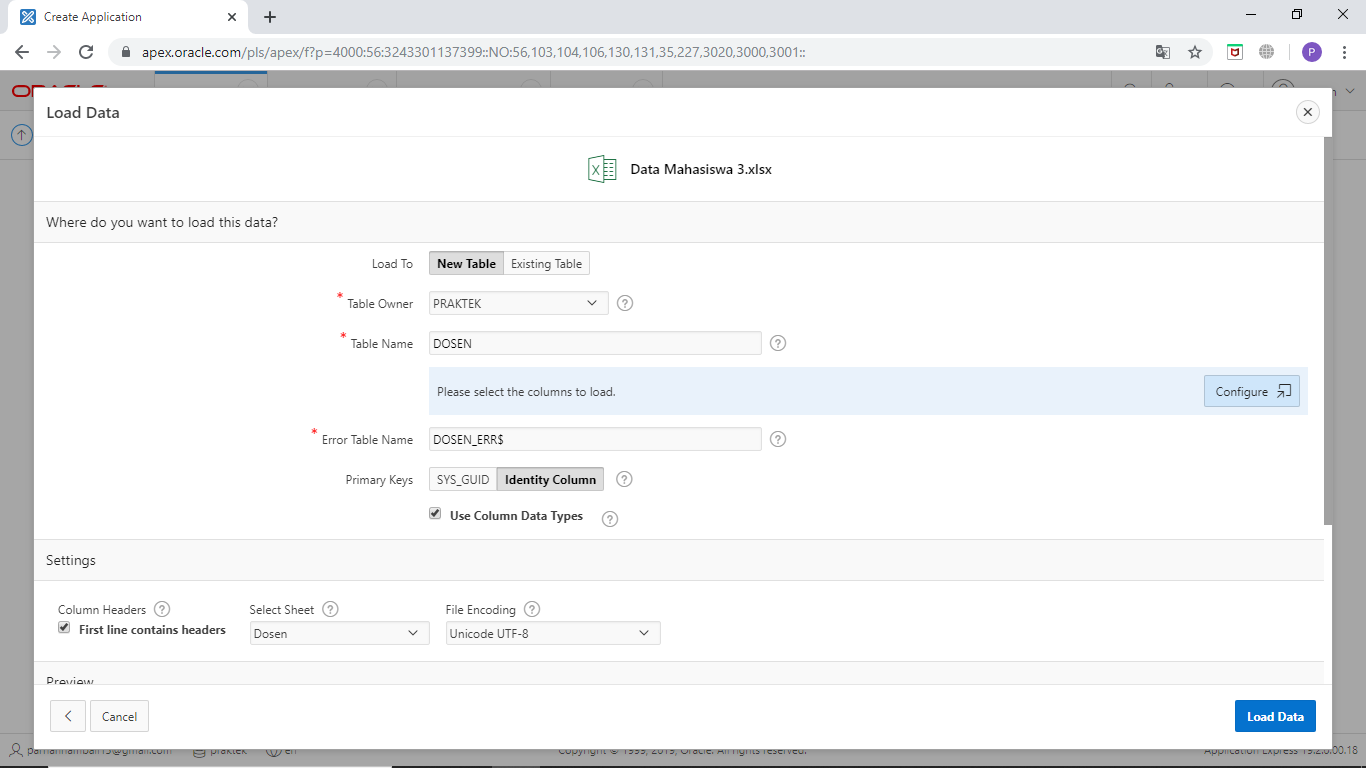
\includegraphics[scale=0.3]{figures/101.png}
    \caption{\textit{Berinama Tabel Dosen}}
    \end{center}
    \label{gambar}
    \end{figure}

\begin{figure}
\item[12]Beri nama sesuai urutan tabel tadi,Selanjutnya beri nama tabel Kuliah,pastikan select sheet nya sesuai dengan penamaan tabelnya. Selanjutnya Load data

    \begin{center}
    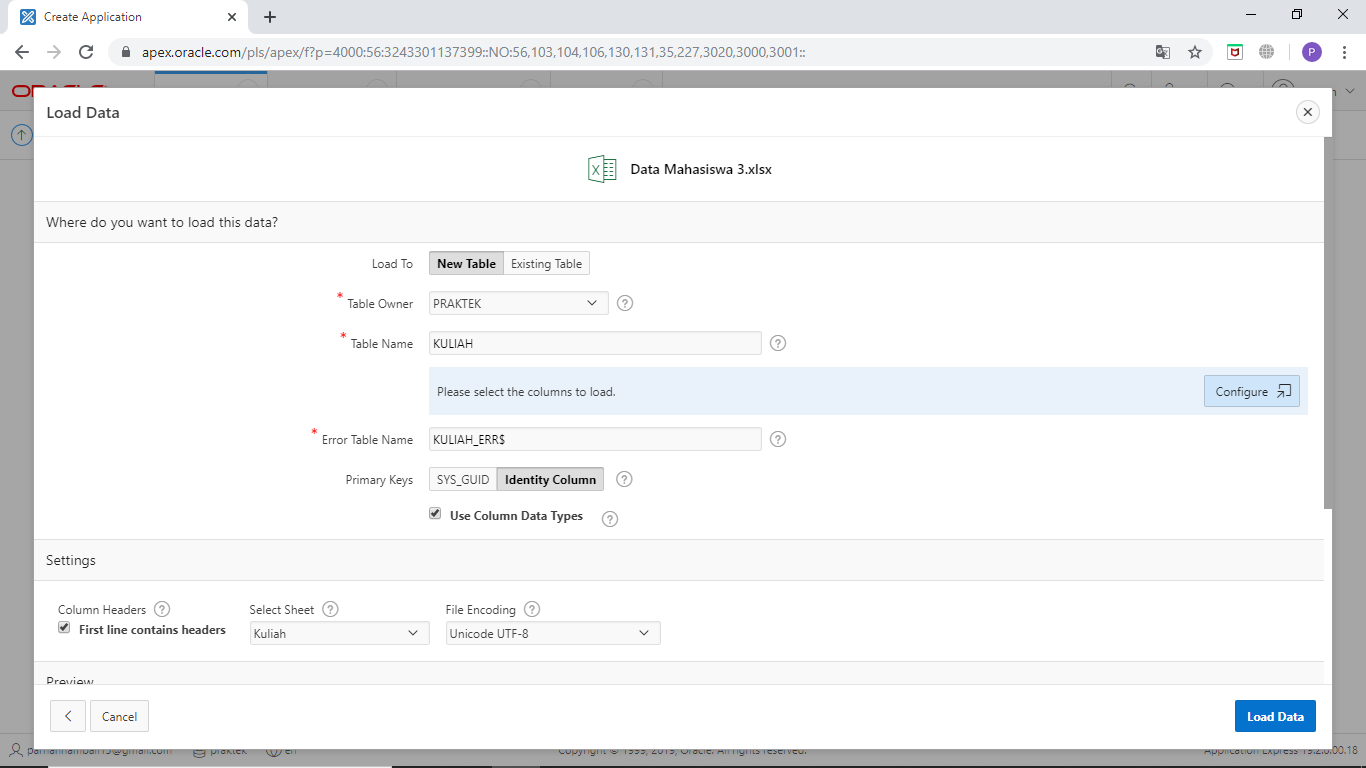
\includegraphics[scale=0.3]{figures/151.png}
    \caption{\textit{Berinama Tabel Kuliah.}}
     \end{center}
    \label{gambar}
    \end{figure}


\begin{figure}
\item[13]Beri nama sesuai urutan tabel tadi,Selanjutnya beri nama tabel Nilai, pastikan select sheet nya sesuai dengan penamaan tabelnya. Selanjutnya Load data

    \begin{center}
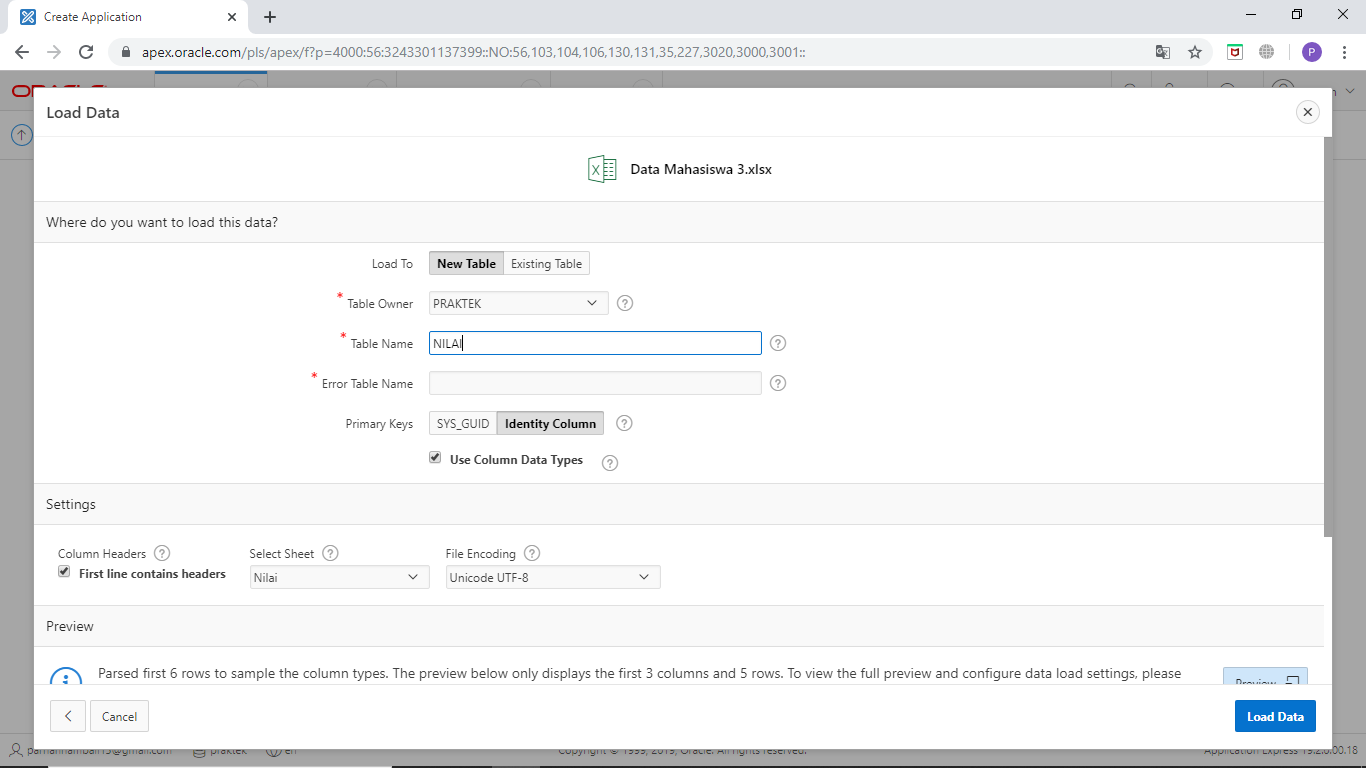
\includegraphics[scale=0.3]{figures/191.png}
    \caption{\textit{Berinama Tabel Nilai.}}
        \end{center}
\label{gambar}
\end{figure}

\begin{figure}
\item[14]Beri nama sesuai urutan tabel tadi,Selanjutnya beri nama tabel Jadwal, pastikan select sheet nya sesuai dengan penamaan tabelnya. Selanjutnya Load data. 

    \begin{center}
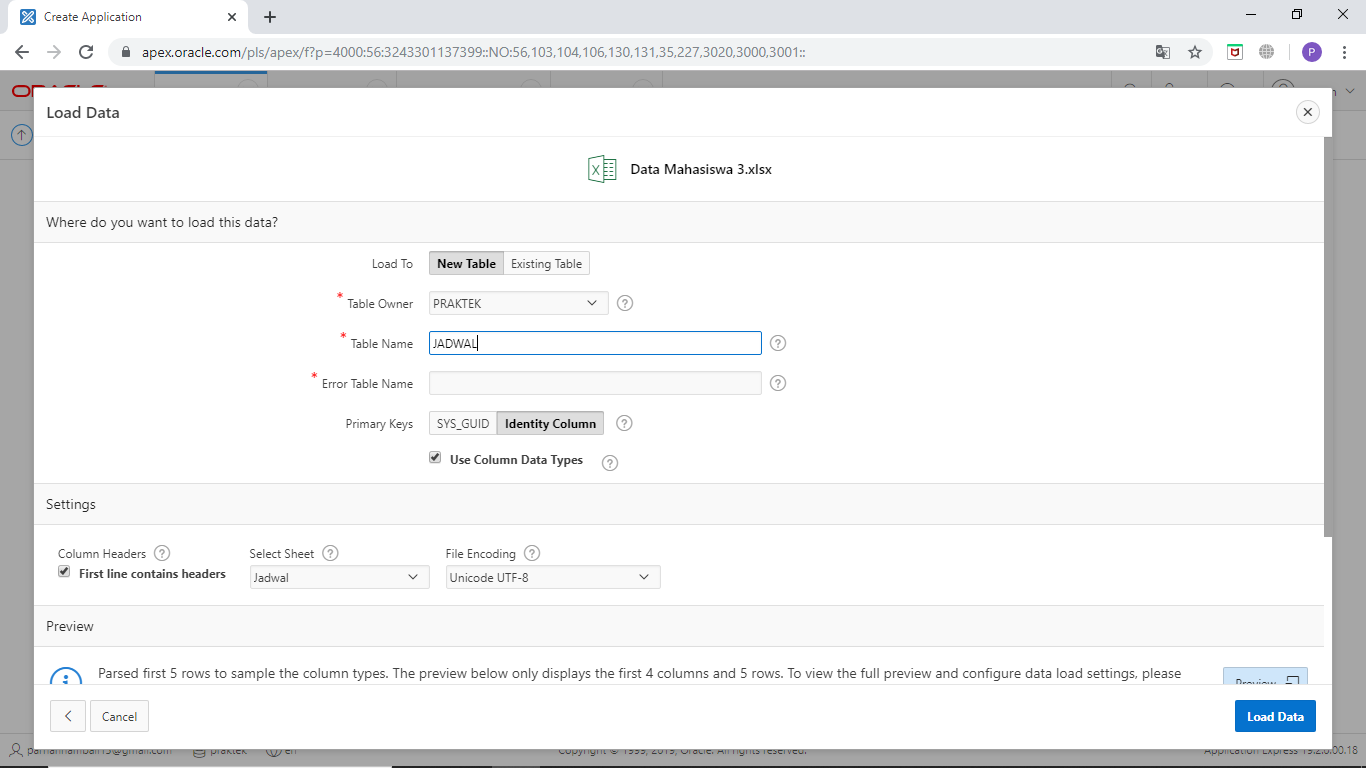
\includegraphics[scale=0.3]{figures/124.png}
    \caption{\textit{Berinama Tabel Jadwal.}}
        \end{center}
\label{gambar}
\end{figure}

\begin{figure}
\item[15]Tabel Telah Berhasil kita buat.

    \begin{center}
    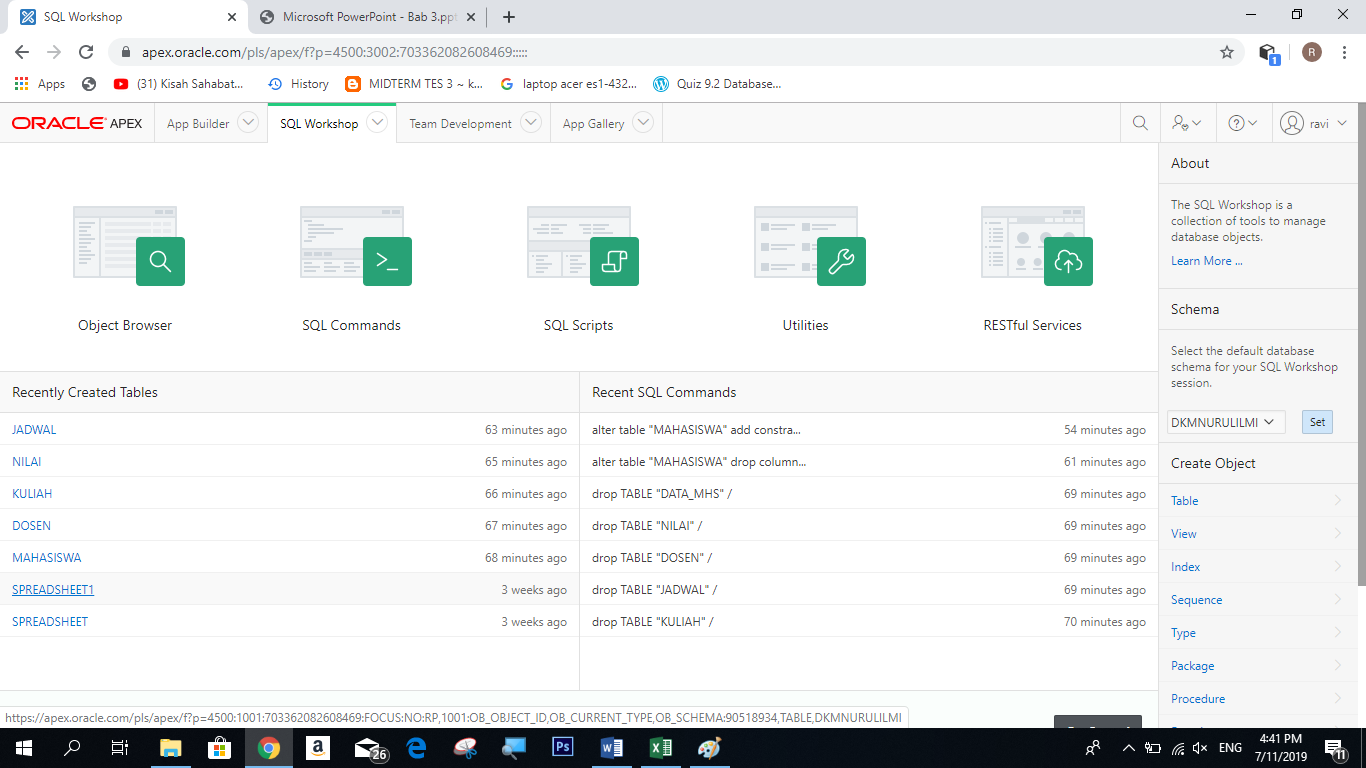
\includegraphics[scale=0.4]{figures/15.png}
    \caption{\textit{Tabel Berhasi Dibuat.}}
    \end{center}
    \label{gambar}
    \end{figure}

\begin{figure}
\item[16]Masuk ke SQL Workshop, Pilih Object Browser, Lalu Hilangkan ID yang berada di semua tabel, baik Nilai,Jadwal,Dosen,Mahasiswa dan Kuliah

    \begin{center}
    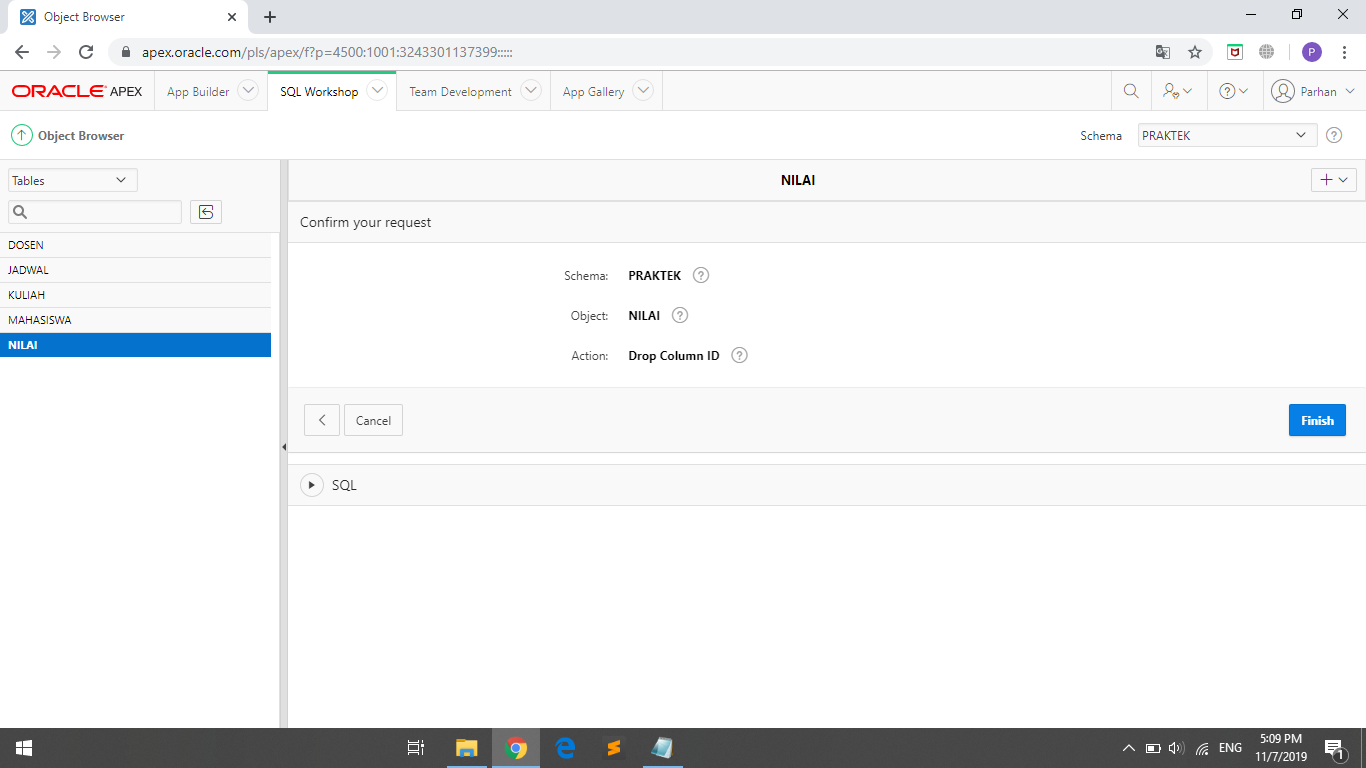
\includegraphics[scale=0.3]{figures/45.png}
    \caption{\textit{Home Object Browser.}}
    \end{center}
    \label{gambar}
    \end{figure}
    
\begin{figure}
\item[17]Pilih Dosen, Clik Constrains, create Jadikan NIK Sebagai Primary Key, Lalu Next. Dan Pilih Kuliah jadikan kode sebagai primary key. Begitu juga dengan Mahasiswa jadikan NIM sebagai Primary Key.

    \begin{center}
    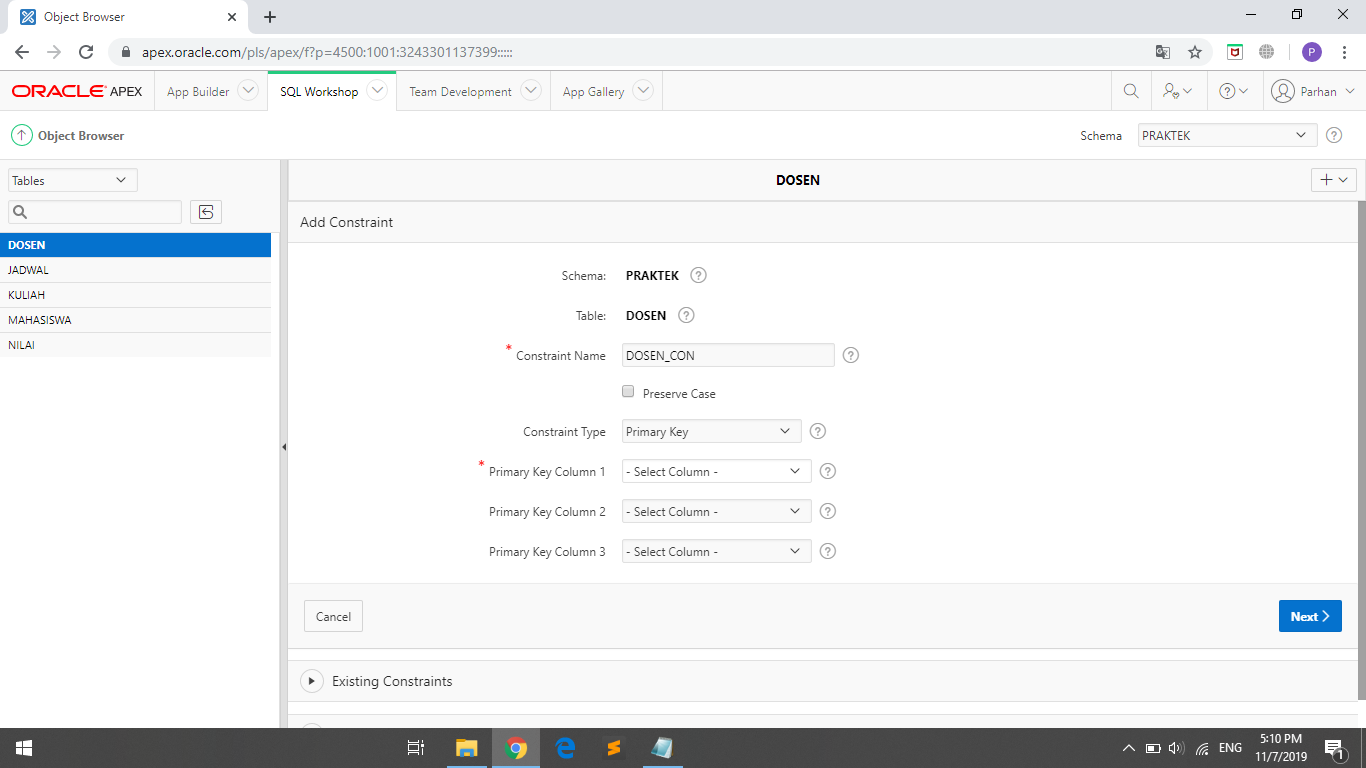
\includegraphics[scale=0.3]{figures/48.png}
    \caption{\textit{Tabel Dosen.}}
    \end{center}
    \label{gambar}
    \end{figure}

\begin{figure}
\item[18]Selanjutnya pilih tabel jadwal,Clik Constrains, create pilih foreign key jadikan kode dengan table name jadwal dan table colum kode.

    \begin{center}
    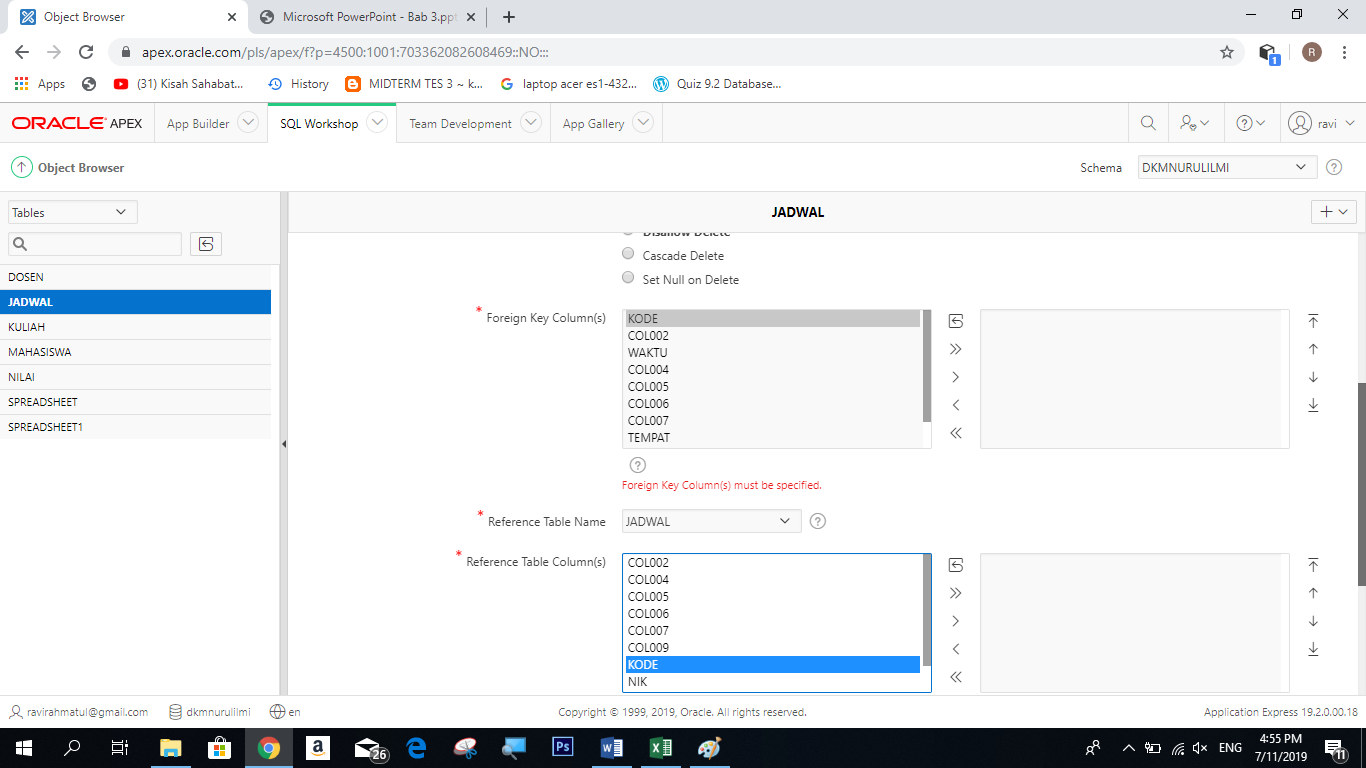
\includegraphics[scale=0.4]{figures/21.png}
    \caption{\textit{Tabel Jadwal.}}
    \end{center}
    \label{gambar}
    \end{figure}

\begin{figure}
\item[19] Selanjutnya pilih tabel Nilai,Clik Constrains, create pilih foreign key jadikan kode dengan table name jadwal dan table colum kode.

    \begin{center}
    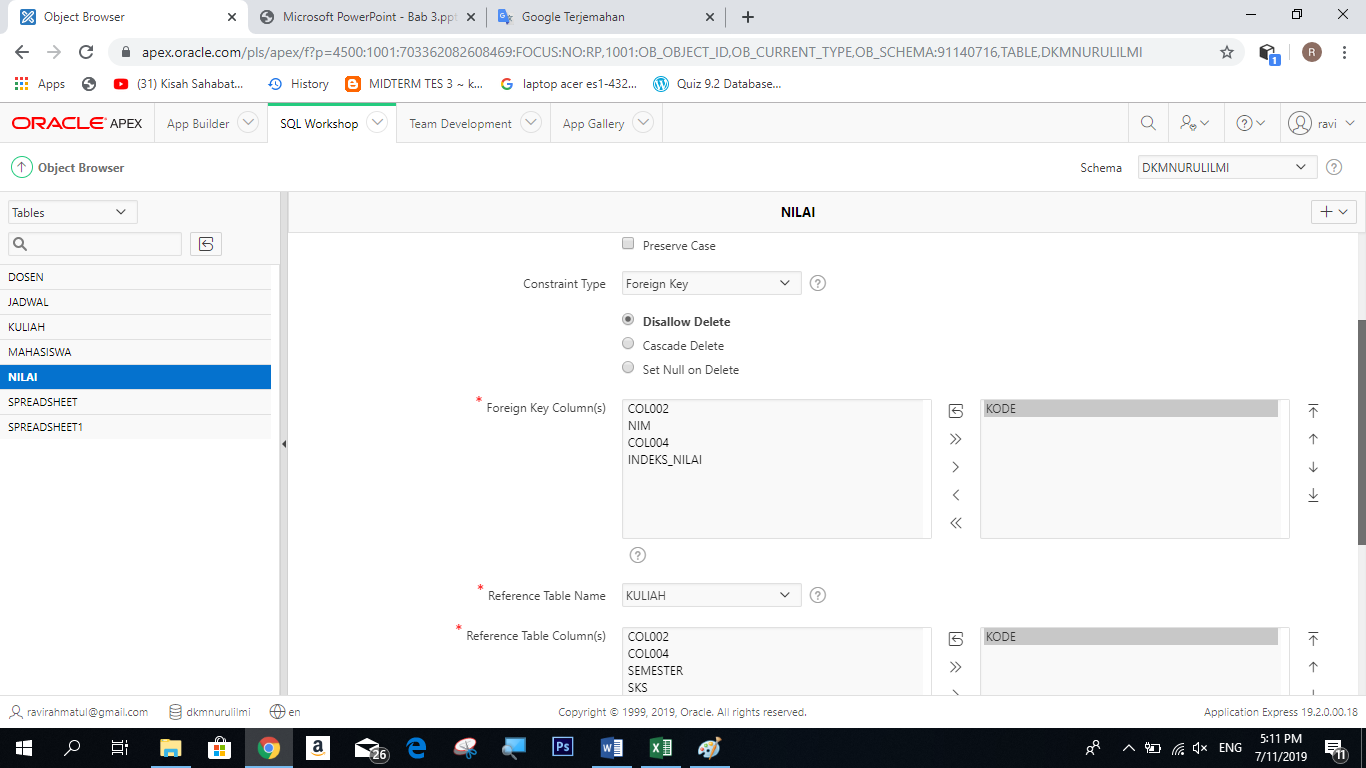
\includegraphics[scale=0.4]{figures/22.png}
    \caption{\textit{Tabel Nilai.}}
    \end{center}
    \label{gambar}
    \end{figure}

\begin{figure}
\item[20] Setelah itu pilih add page, interaktive report, Berinama tabel Mahasiswa seperti gambar dibawah ini. Begitu juga dengan Dosen, Kuliah, Nilai dan Jadwal

    \begin{center}
    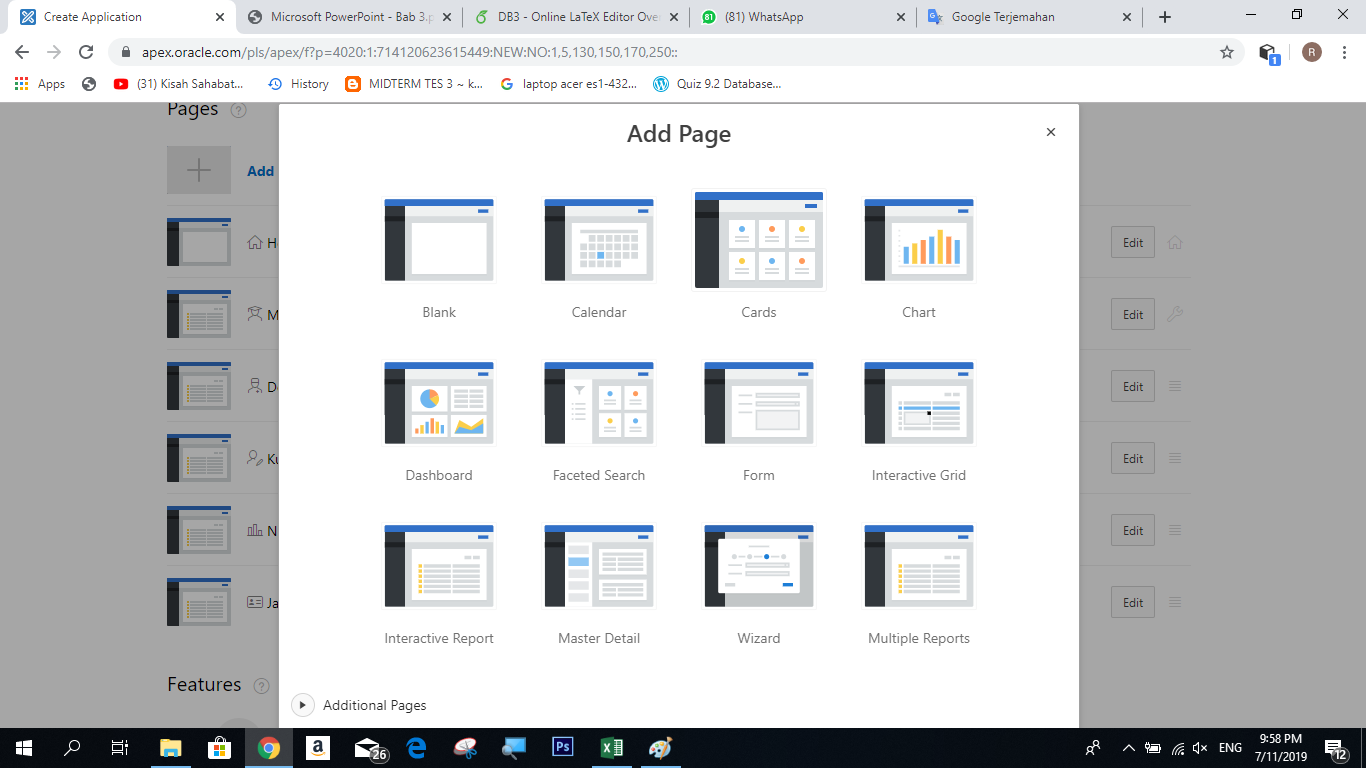
\includegraphics[scale=0.4]{figures/24.png}
    \caption{\textit{Add Page.}}
    \end{center}
    \label{gambar}
    \end{figure}    

\begin{figure}
\item[21] Setelah itu pilih add page, interaktive report, Berinama tabel Mahasiswa seperti gambar dibawah ini. Begitu juga dengan Dosen, Kuliah, Nilai dan Jadwal. Selanjutnya Create Application, jangan lupa memberi nama aplikasi yang ingin kita buat ini.

    \begin{center}
    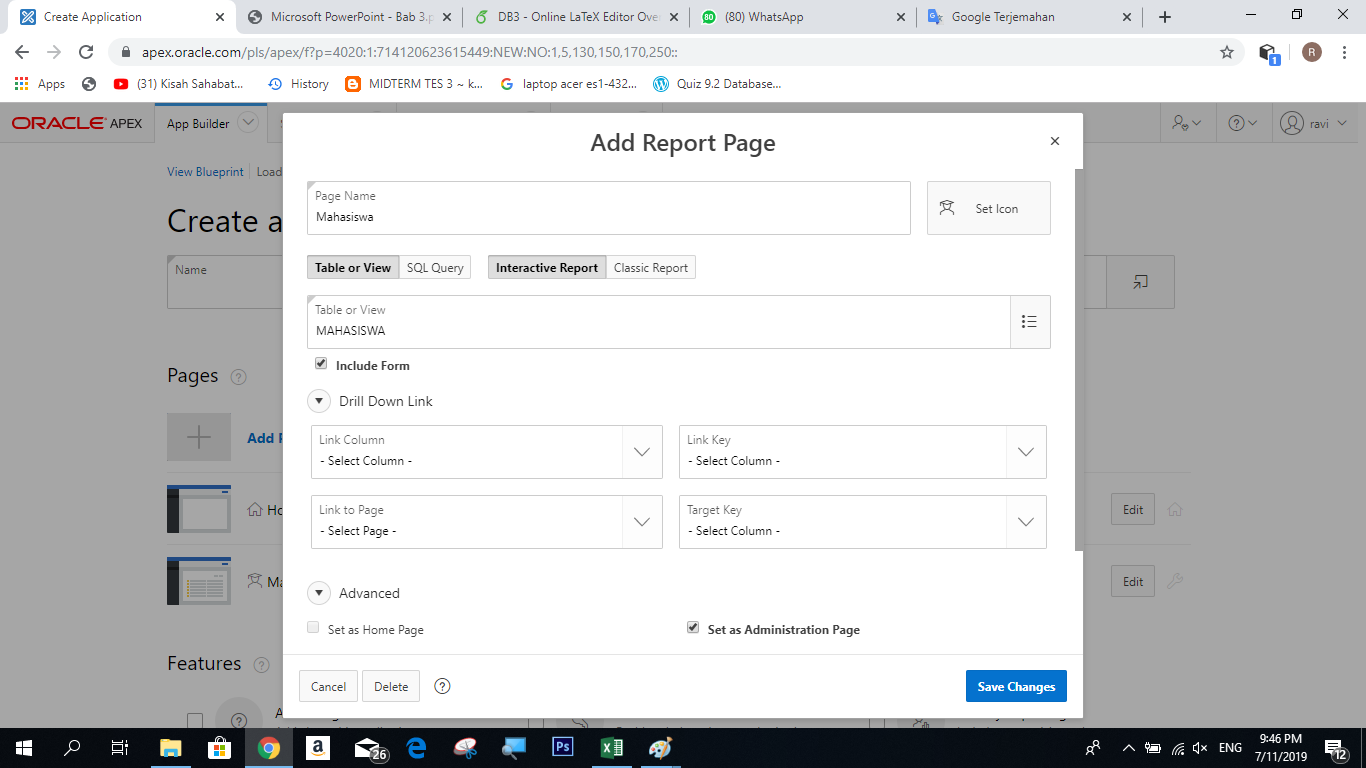
\includegraphics[scale=0.4]{figures/25.png}
    \caption{\textit{Add Page.}}
    \end{center}
    \label{gambar}
    \end{figure}    

\begin{figure}
\item[22]Tunggu Beberapa saat

    \begin{center}
    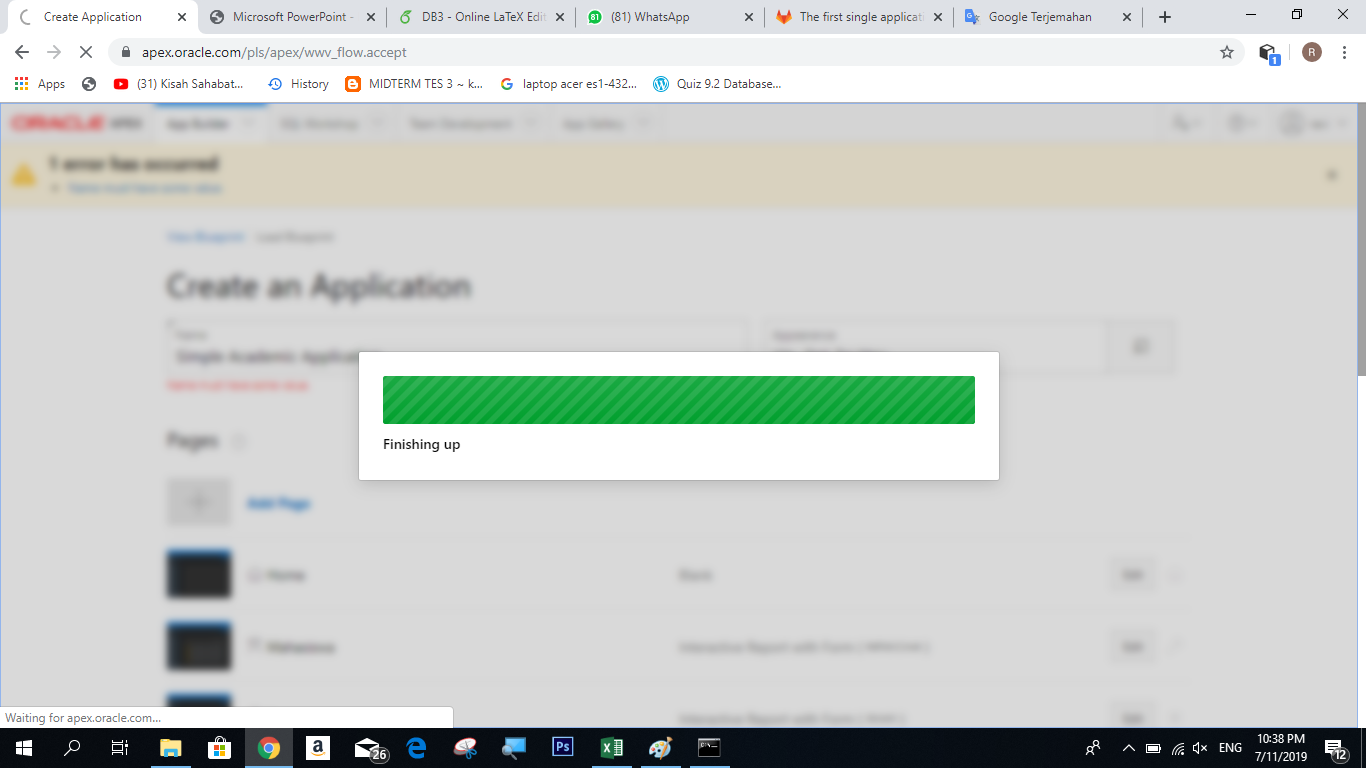
\includegraphics[scale=0.4]{figures/26.png}
    \caption{\textit{Loading.}}
    \end{center}
    \label{gambar}
    \end{figure}   

\begin{figure}
\item[23]Selanjutnya kita Login dengan menggunakan email dan password kita

    \begin{center}
    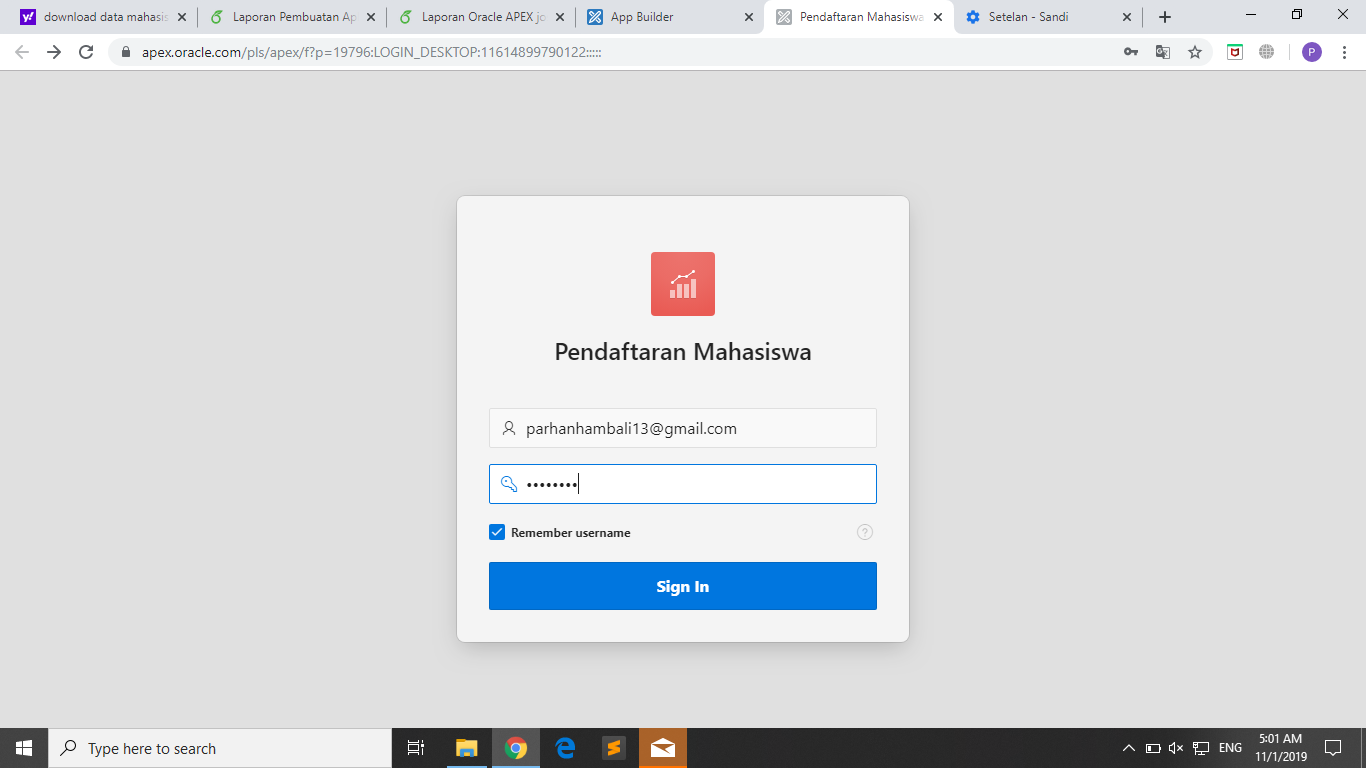
\includegraphics[scale=0.3]{figures/32.png}
    \caption{\textit{Login.}}
    \end{center}
    \label{gambar}
    \end{figure}   

\begin{figure}
\item[24]Aplikasi Akademik Sederhana kita telah selesai dibuat. Didalam aplikasi ini kita dapat mencari data dan menambah data yang kita inginkan.
Username/email : parhanhambali13@gmail.com
password : Asus123 (dedepan Asus Memakai pagar Menjadi pagarAsus123)
Link App : https://apex.oracle.com/pls/apex/f?p=35515:1:106951913872956::NO:::

    \begin{center}
    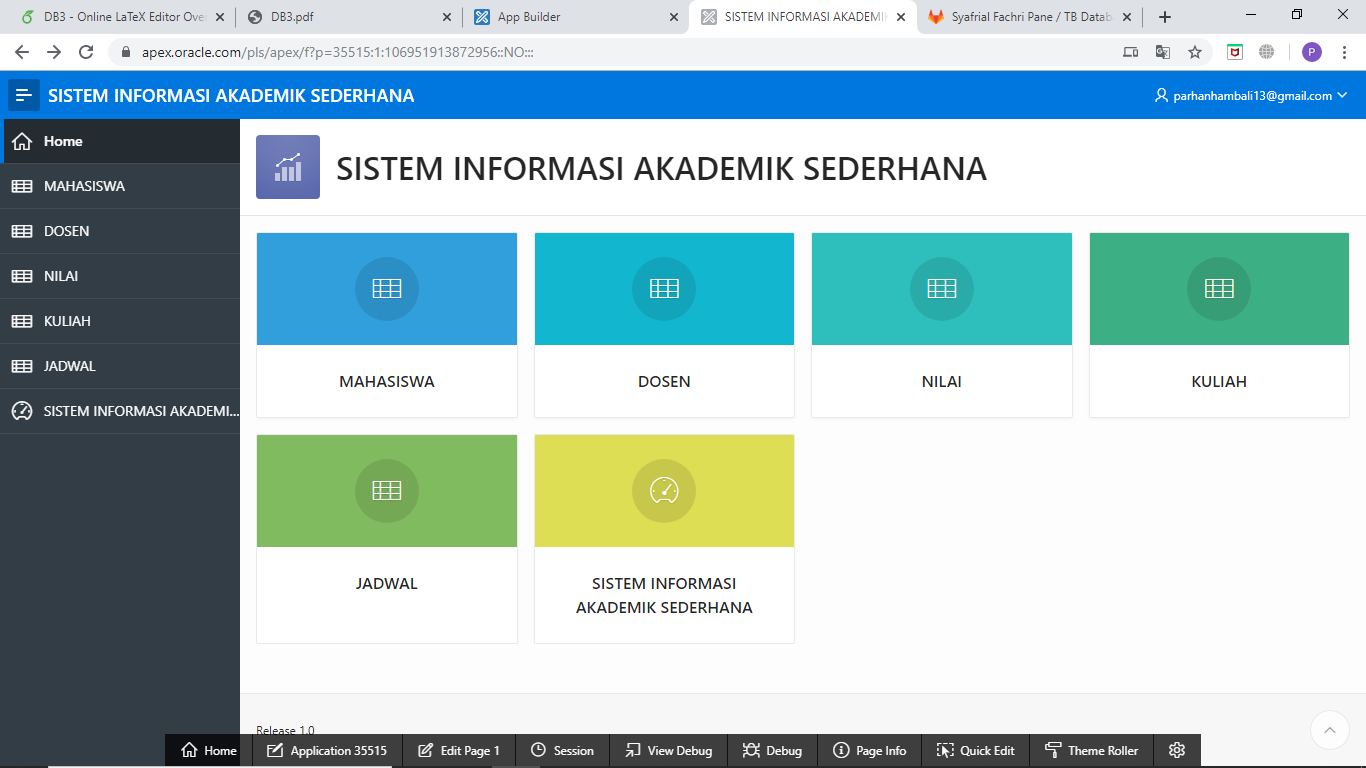
\includegraphics[scale=0.3]{figures/29.png}
    \caption{\textit{Home App Akademik Sederhana.}}
    \end{center}
    \label{gambar}
    \end{figure}   

\end{enumerate}
